\section{Evaluation}

% Provide an introductory paragraph that summarizes what's in this section: a list of runs/experiments intended to test your implementation and ideas. Describe each of these experiments in a few words/a sentence.

To evaluate the impact of different memory access patterns on performance, we conducted a series of experiments using the three sum computation methods. For each method, we measured the elapsed time and computed key performance metrics such as MFLOP/s, memory bandwidth utilization, and memory latency. These metrics allow us to understand how efficiently each method uses computational resources and memory subsystems under varying access patterns.
 

\subsection{Computational Platform and Software Environment}
% What machine did you run your tests on? What was the processor, its clock rate (GHz), size of L1/L2/L3 cache, how much memory (DRAM), what OS?
The experiments were conducted on the Perlmutter supercomputer at NERSC. The key specifications are summarized in Table~\ref{tab:machine_detail}.

We used \textit{gcc version 7.5.0 (SUSE Linux)} as the C++ compiler. For optimization, the following compiler flags were applied: \textit{-O3 -DNDEBUG -Wall -pedantic -march=native}, aiming for maximum speed and strict standard compliance. Additionally, to assess the impact of compiler optimizations, we tested with the \textit{-O0} flag, which disables optimizations, to provide a baseline for performance comparison.

\begin{table}[htbp]
    \centering\small
    \begin{tabular}{c|c}
        \textbf{Specification} & \textbf{Details} \\
        \hline
        CPU & AMD EPYC 7763 (Milan) \cite{nersc_perlmutter_architecture} \\
        Instruction Set & AVX2 instruction set  \cite{nersc_perlmutter_architecture} \\
        Number of Cores & 64 \cite{nersc_perlmutter_architecture} \\
        Clock Rate & 2.45 GHz \cite{nersc_perlmutter_architecture} \\
        L1 Cache & 32 KB per core \cite{amd_epyc_tuning_guide} \\
        L2 Cache & 512 KB per core \cite{amd_epyc_tuning_guide} \\
        L3 Cache & 32 MB shared among 8 cores  \cite{amd_epyc_tuning_guide} \\
        DRAM & 512 GB DDR4 \cite{nersc_perlmutter_architecture} \\
        Memory Bandwidth & 204.8 GB/s per CPU \cite{nersc_perlmutter_architecture} \\
        Max Memory Channels & 8 per socket \cite{amd_epyc_tuning_guide} \\
        Computational Throughput & 39.2 GFLOPS per core \cite{nersc_perlmutter_architecture} \\
        Operating System & x86\_64 GNU/Linux \\
    \end{tabular}
    \caption{Specifications of the Computational Platform Used for Experiments}
    \label{tab:machine_detail}
\end{table}

\FloatBarrier
\subsection{Methodology}
\label{sec:methodology}

% Describe the procedures you use to test your system.
% Performance metrics: describe exactly what metrics you employ to measure performance. It might be elapsed time from instrumentation code you added around the main computational code. Later in the term, it may be something else.
% Experimental design: did you run tests over a set of prescribed problem sizes? If so, what were they?
We evaluated the performance of different summation methods using problem sizes of \(2^{23}\), \(2^{24}\), \(2^{25}\), \(2^{26}\), \(2^{27}\), and \(2^{28}\). Performance was measured by calculating the elapsed time using an instrumentation code placed around the main summation code, as shown in Listing~\ref{listing:measuring-elapsed-time}. From the elapsed time, we derived three key performance metrics:

\begin{itemize}
    \item \textbf{MFLOP/s}: Measures computational throughput as operations per second, calculated as:
    \begin{itemize}
        \item \textit{MFLOP/s} = \(\frac{\text{ops}}{\text{time}}\)
        \item \textit{ops} = number of operations / \(1M\)
        \item \textit{time} = runtime (seconds)
    \end{itemize}
    
    \item \textbf{Memory Bandwidth Utilization (\%)}: The percentage of theoretical peak memory bandwidth used, computed by:
    \begin{itemize}
        \item \% \textit{Memory Bandwidth} = \(\frac{\text{bytes/time}}{\text{capacity}} \times 100\)
        \item \textit{bytes} = number of memory bytes accessed
        \item \textit{time} = runtime (seconds)
        \item \textit{capacity} = theoretical peak memory bandwidth of the system (see Table~\ref{tab:machine_detail})
        \item Since the direct sum method does not access memory, its memory bandwidth utilization is consistently \(0\%\). 
    \end{itemize}
    
    \item \textbf{Average Memory Latency}: Measures the average time per memory access, defined as:
    \begin{itemize}
        \item \textit{Avg Memory Latency} = \(\frac{\text{time}}{\text{accesses}}\)
        \item \textit{time} = runtime (seconds)
        \item \textit{accesses} = number of memory accesses by the program
        \item Since the direct sum method does not access memory, its memory latency is consistently \(0\). 
    \end{itemize}
\end{itemize}

\begin{lstlisting}[caption={Measuring Elapsed Time: },label={listing:measuring-elapsed-time}, name=measuring-elapsed-time, float=htbp, style=mystyle,language=C++]
for (int64_t n : problem_sizes)
{
    setup(n, &A[0]);
    
    start_time = get_current_time();    
    result = sum(n, &A[0]);
    end_time = get_current_time();

    elapsed_time = end_time - start_time;
}
\end{lstlisting}

\subsection{Experiment: MFLOP/s}
% Describe the experiment in a few sentences: what question are you trying to answer, what problem sizes/etc did you use (it's ok to make reference back to Sec.~\ref{sec:methodology} so you don't have to repeat a lot of details. 

% Present the results of your experiment using either tabular forms of information, such as in Table~\ref{tab:MyTable1}, or using charts and graphs as in Fig.~\ref{fig:MyPlot1}.

In this experiment, we aimed to evaluate the computational throughput (MFLOP/s) for different memory access patterns. The configuration details for this experiment are provided in Sec.~\ref{sec:methodology}. The results are summarized in Table~\ref{tab:mflops-o0} and Table~\ref{tab:mflops-o3}, and visualized in Fig.~\ref{fig:MFLOPs_O0} and Fig.~\ref{fig:MFLOPs_O3}.

The results show that the MFLOP/s is significantly higher with the \textit{-O3} optimization flag compared to \textit{-O0}. The direct sum method achieved the highest MFLOP/s, while the vector sum, though less efficient than the direct sum, performed much better than the indirect sum. The performance of the direct sum and vector sum methods remained relatively stable across different problem sizes, whereas the MFLOP/s of the indirect sum method decreased as the problem size increased.

\begin{figure}[htbp]
    \centering
    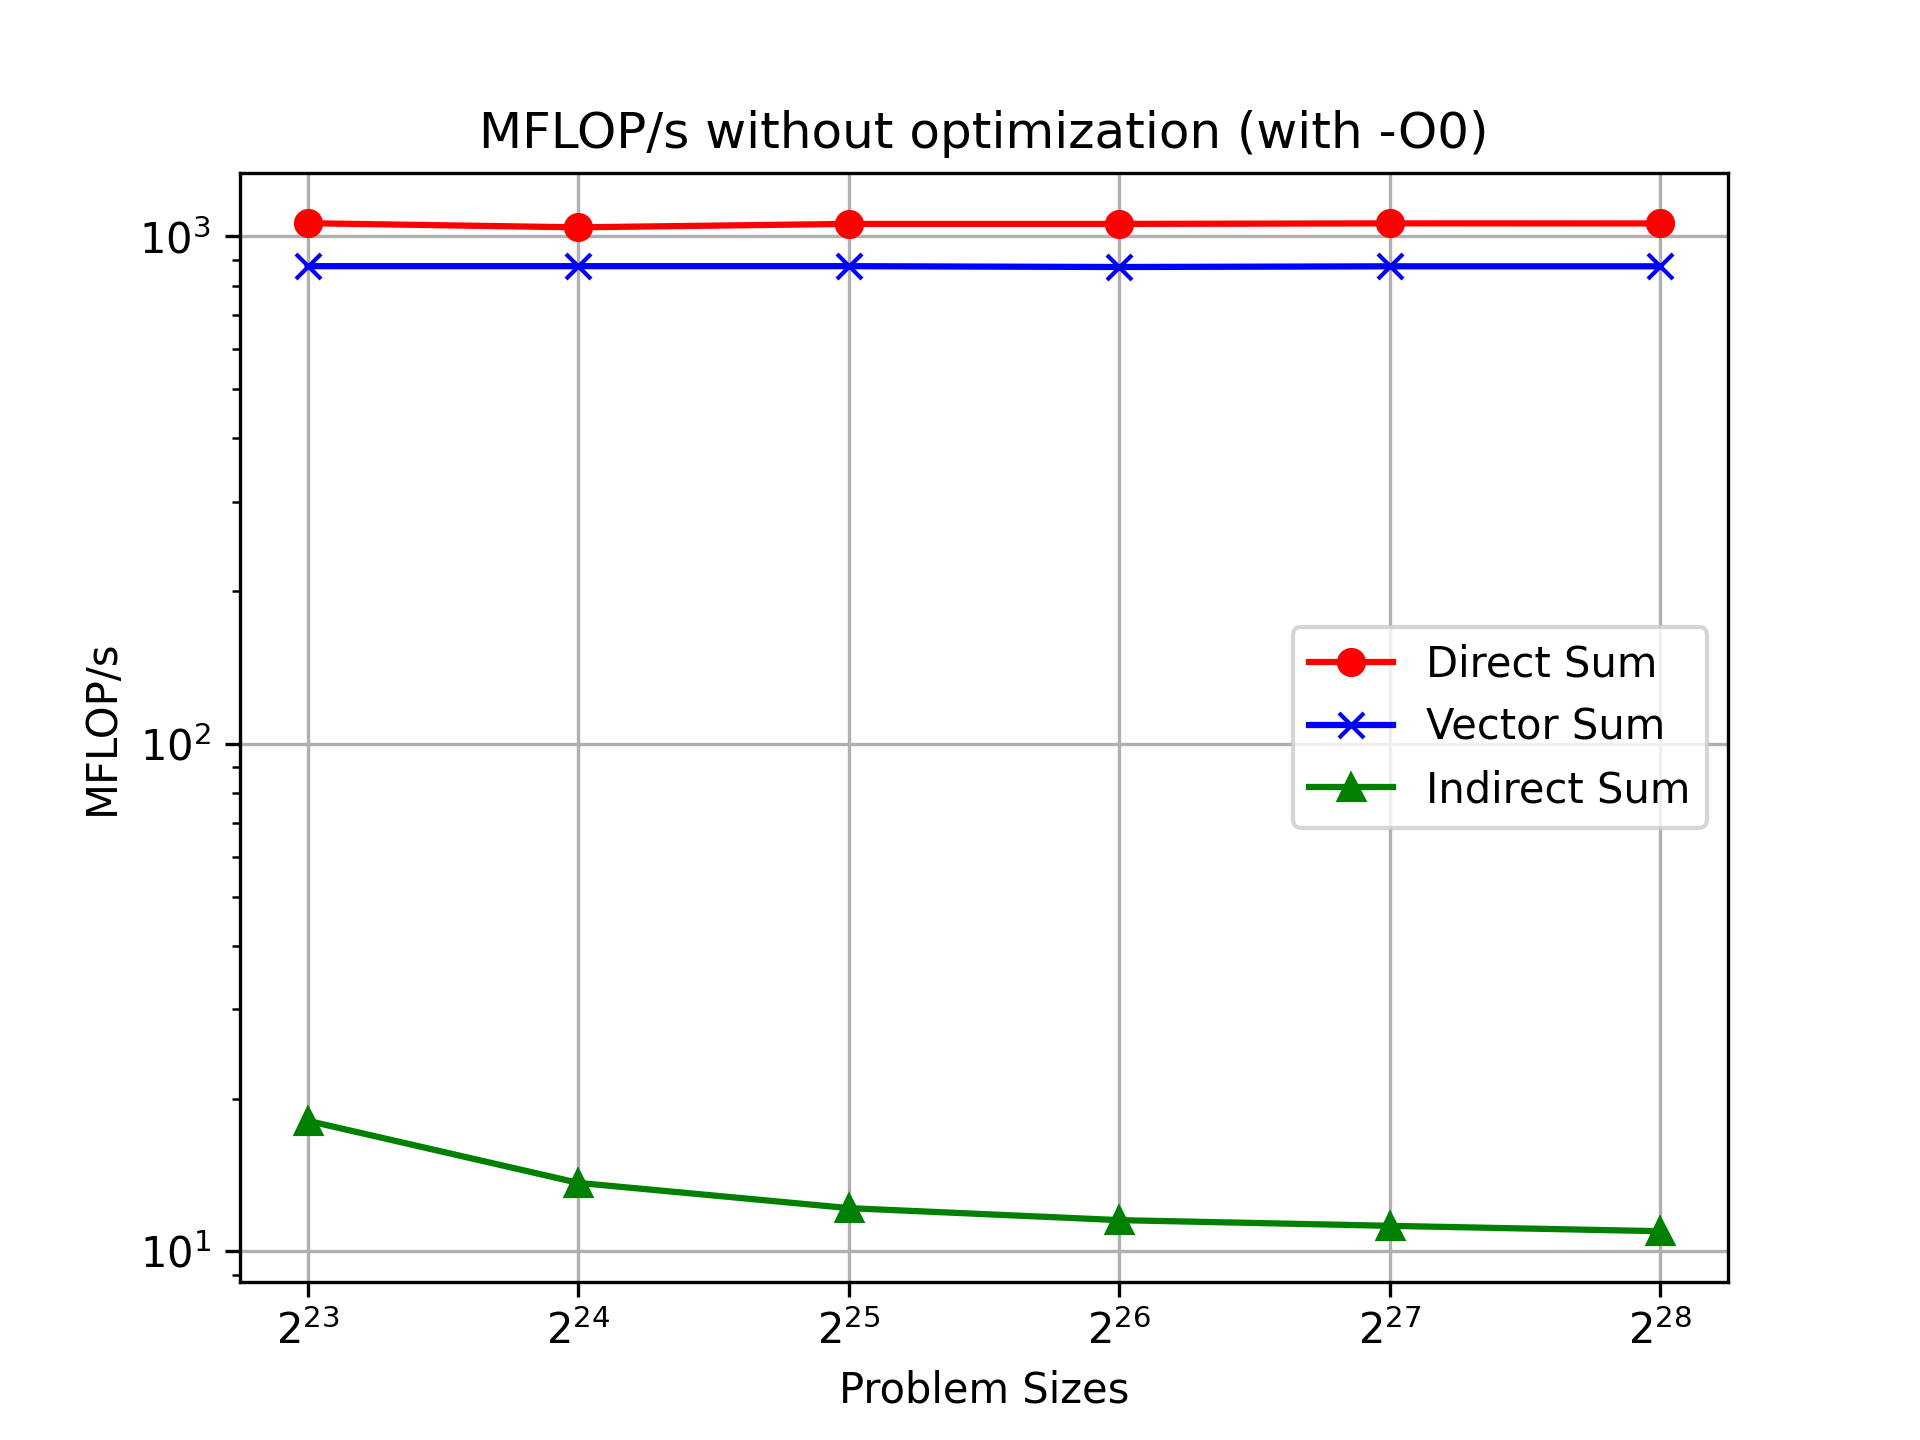
\includegraphics[width=0.45\textwidth]{MFLOPs_O0.png}
    \caption{MFLOP/s without optimization (\textit{-O0}).}
    \label{fig:MFLOPs_O0}
\end{figure}

\begin{figure}[htbp]
    \centering
    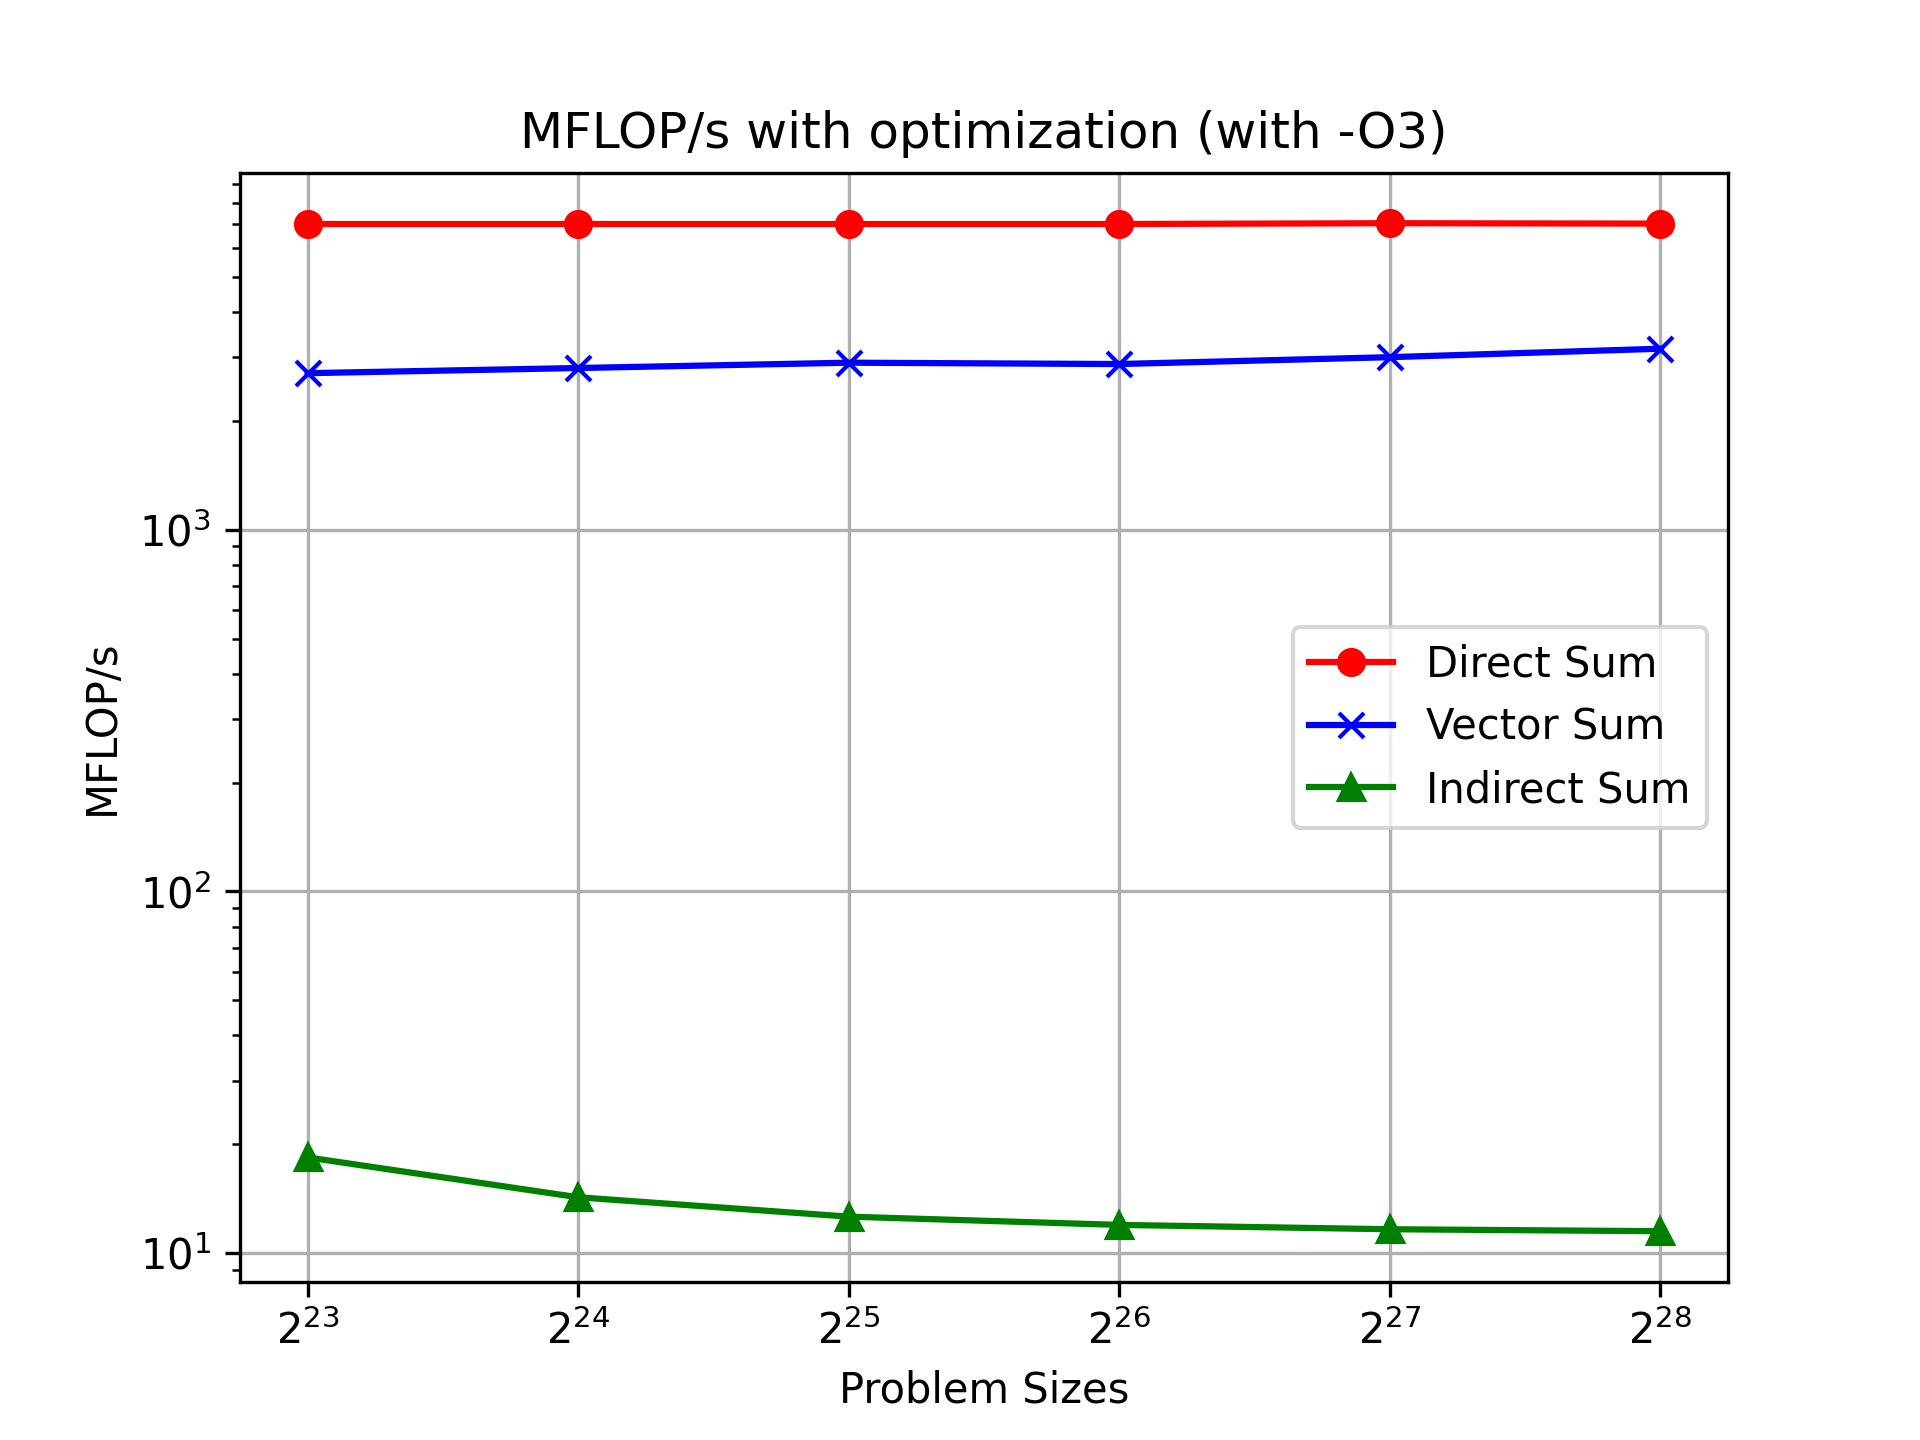
\includegraphics[width=0.45\textwidth]{MFLOPs_O3.png}
    \caption{MFLOP/s with optimization (\textit{-O3}).}
    \label{fig:MFLOPs_O3}
\end{figure}

\begin{table}[htbp]
    \centering\small
    \begin{tabular}{c|cll}
 Problem Size (N) & Direct Sum & Vector Sum & Indirect Sum \\ \hline
 $2^{23}$ & 1,061.8& 873.8&18.1\\
 $2^{24}$ & 1,042.1& 873.8&13.7\\
 $2^{25}$ & 1,058.5& 873.8&12.2\\
 $2^{26}$ & 1,058.5& 870.4&11.5\\
 $2^{27}$ & 1,061.0& 873.2&11.2\\
 $2^{28}$ & 1,060.6& 873.2&11.0\\ 
    \end{tabular}
    \caption{MFLOP/s without optimization (with \textit{-O0})}
    \label{tab:mflops-o0}
    \begin{tabular}{c|cll}
 Problem Size (N) & Direct Sum & Vector Sum & Indirect Sum \\ \hline
 $2^{23}$ & 6,990.5& 2,706.0&18.4\\
 $2^{24}$ & 6,990.5& 2,796.2&14.3\\
 $2^{25}$ & 6,990.5& 2,892.6&12.6\\
 $2^{26}$ & 6,990.5& 2,867.9&12.0\\
 $2^{27}$ & 7,027.1& 2,995.9&11.7\\
 $2^{28}$ & 7,008.8& 3,161.8&11.5\\ 
    \end{tabular}
    \caption{MFLOP/s with optimization (with \textit{-O3})}
    \label{tab:mflops-o3}
\end{table}

\subsection{Experiment: Memory Bandwidth Utilization (\%)}
In this experiment, we evaluated the memory bandwidth utilization for each memory access pattern. The configuration details for this experiment are provided in Sec.~\ref{sec:methodology}. The results are summarized in Table~\ref{tab:memory-bandwidth-o0} and Table~\ref{tab:memory-bandwidth-o3}, and visualized in Fig.~\ref{fig:Bandwidth_O0} and Fig.~\ref{fig:Bandwidth_O3}.

Since the direct sum method does not access memory, its memory bandwidth utilization is consistently \(0\%\). The results indicate that, without optimization (using \textit{-O0}), the memory bandwidth utilization for the vector sum method remains stable across different problem sizes, while it slightly decreases for the indirect sum method as the problem size increases. With optimization (using \textit{-O3}), a similar decreasing trend is observed for the indirect sum method, whereas the bandwidth utilization for the vector sum method increases as the problem size grows.
\begin{figure}[htbp]
    \centering
    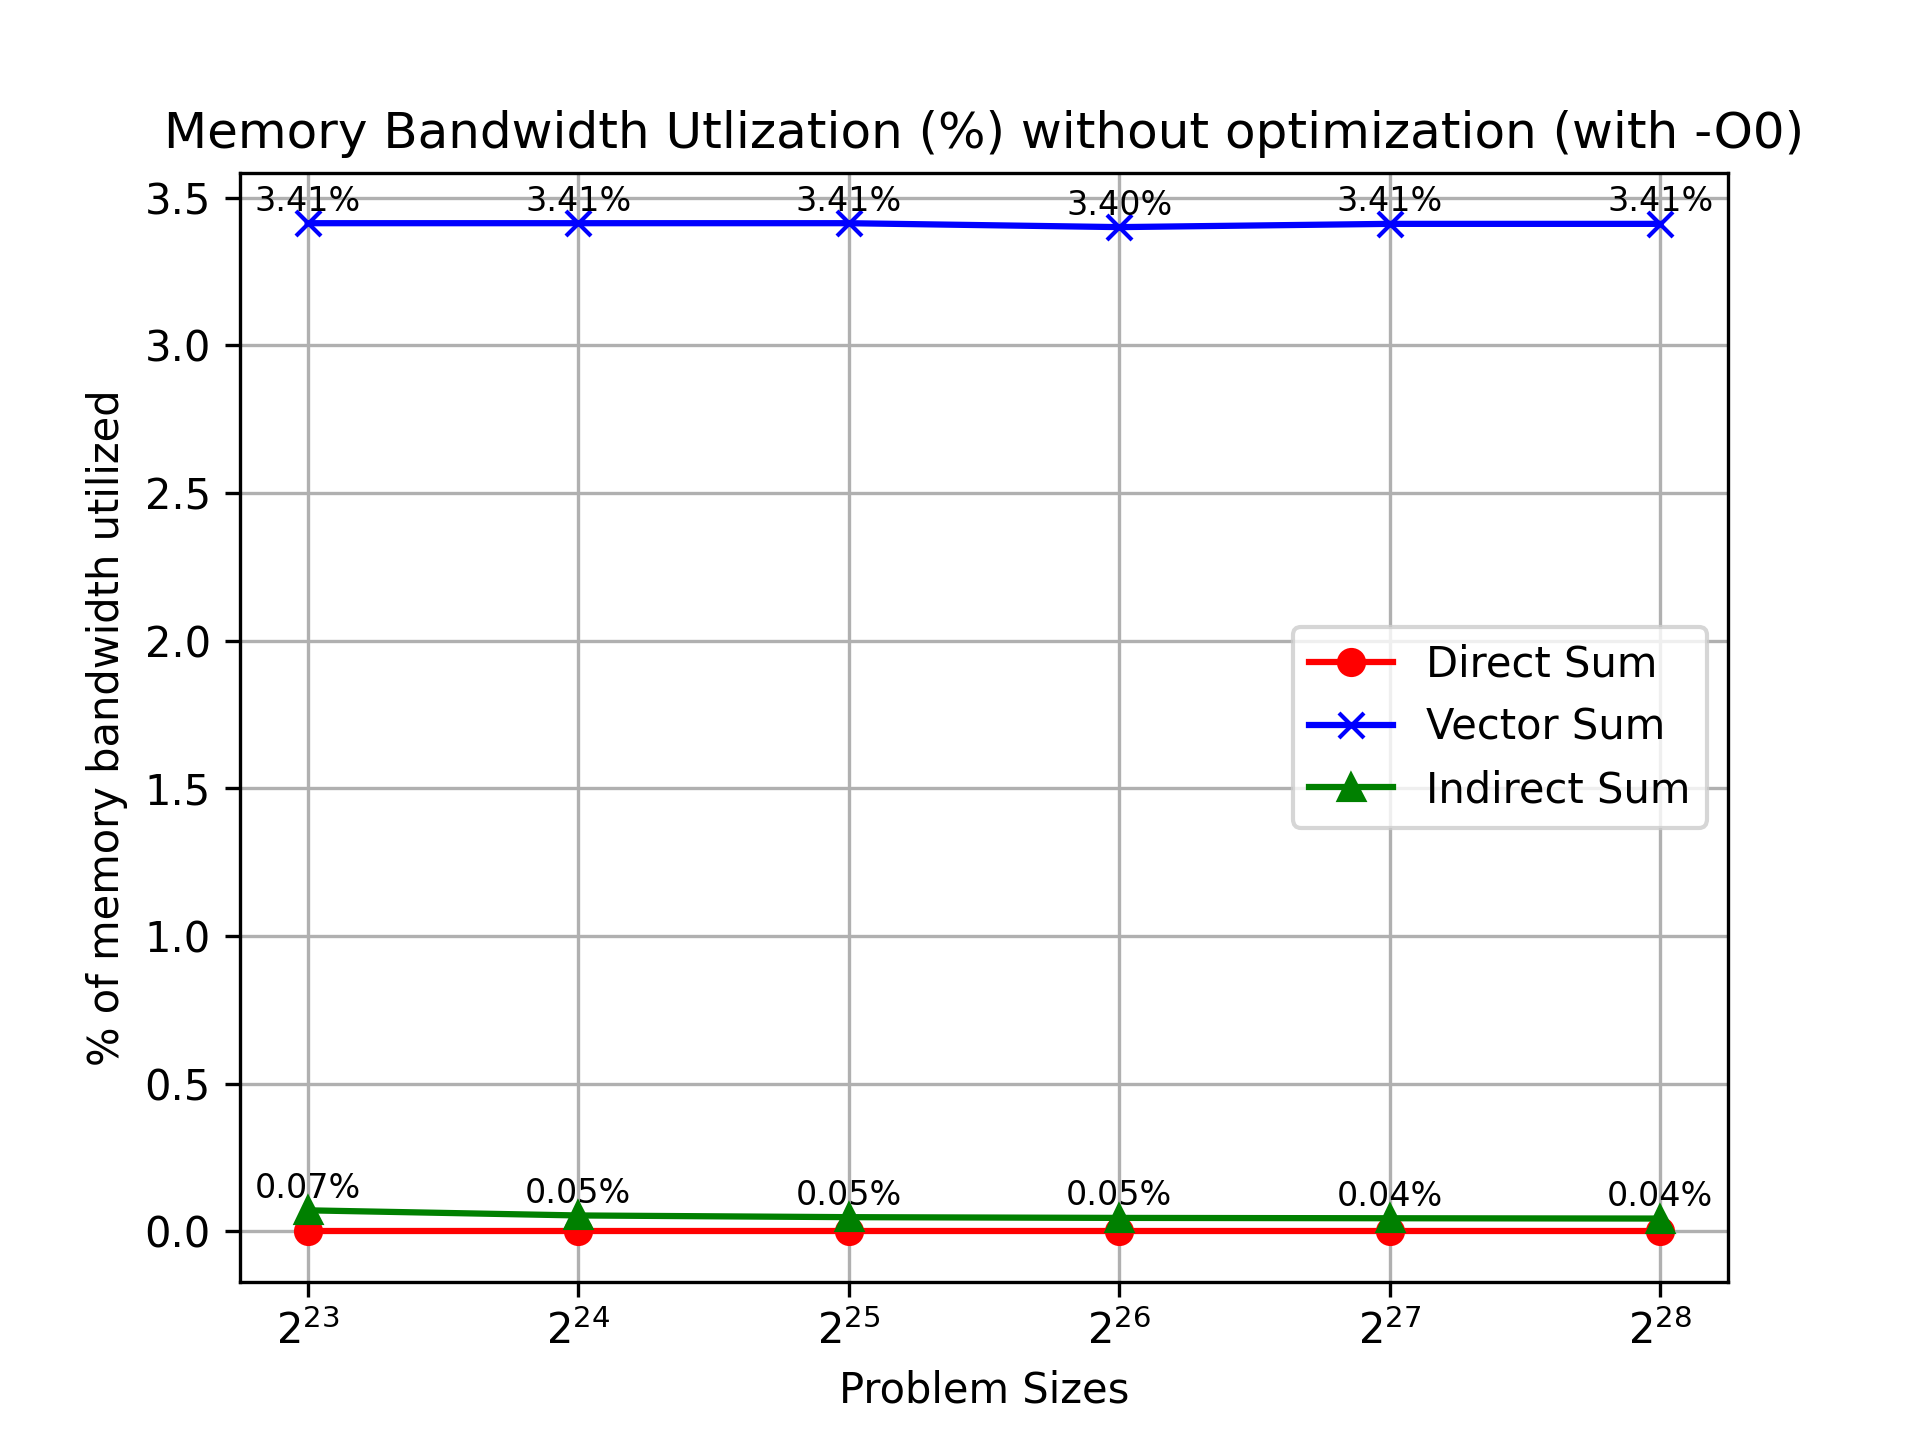
\includegraphics[width=0.45\textwidth]{Bandwidth_O0.png}
    \caption{Memory Bandwidth Utilization (\%) without optimization (\textit{-O0}).}
    \label{fig:Bandwidth_O0}
\end{figure}

\begin{figure}[htbp]
    \centering
    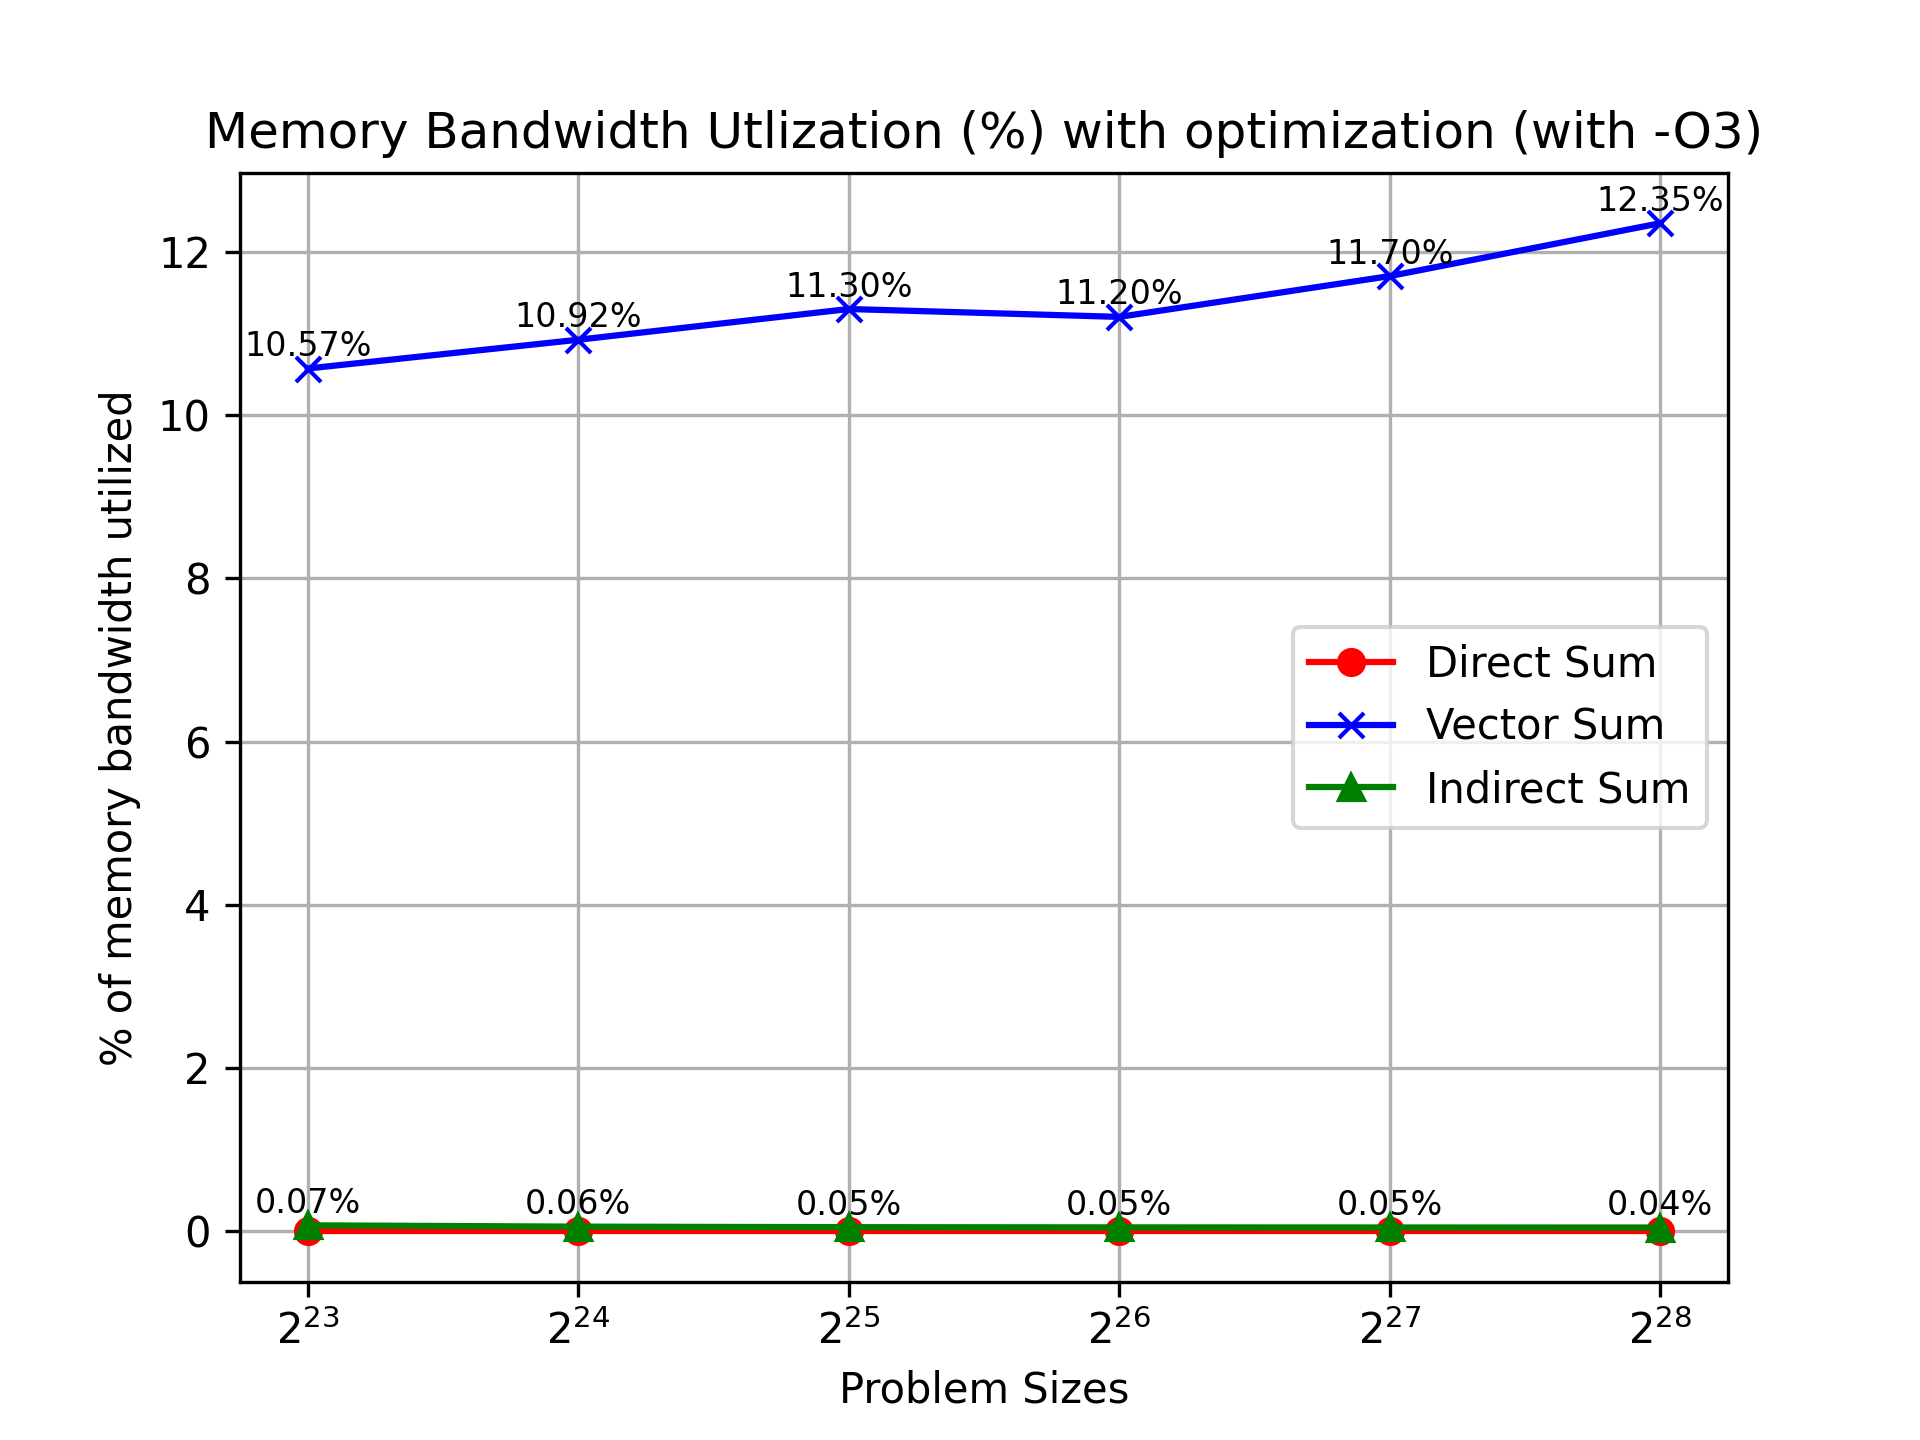
\includegraphics[width=0.45\textwidth]{Bandwidth_O3.png}
    \caption{Memory Bandwidth Utilization (\%) with optimization (\textit{-O3}).}
    \label{fig:Bandwidth_O3}
\end{figure}

\begin{table}[htbp]
    \centering\small
    \begin{tabular}{c|cll}
 Problem Size (N) & Direct Sum & Vector Sum & Indirect Sum \\ \hline
 $2^{23}$ & 0\%& 3.41\%&0.07\%\\
 $2^{24}$ & 0\%& 3.41\%&0.05\%\\
 $2^{25}$ & 0\%& 3.41\%&0.05\%\\
 $2^{26}$ & 0\%& 3.40\%&0.05\%\\
 $2^{27}$ & 0\%& 3.41\%&0.04\%\\
 $2^{28}$ & 0\%& 3.41\%&0.04\%\\ 
    \end{tabular}
    \caption{Memory Bandwidth Utilization (\%) without optimization (with \textit{-O0})}
    \label{tab:memory-bandwidth-o0}
    \begin{tabular}{c|cll}
 Problem Size (N) & Direct Sum & Vector Sum & Indirect Sum \\ \hline
 $2^{23}$ & 0\%& 10.57\%&0.14\%\\
 $2^{24}$ & 0\%& 10.92\%&0.11\%\\
 $2^{25}$ & 0\%& 11.30\%&0.10\%\\
 $2^{26}$ & 0\%& 11.20\%&0.09\%\\
 $2^{27}$ & 0\%& 11.70\%&0.09\%\\
 $2^{28}$ & 0\%& 12.35\%&0.09\%\\ 
    \end{tabular}
    \caption{Memory Bandwidth Utilization (\%) with optimization (with \textit{-O3})}
    \label{tab:memory-bandwidth-o3}
\end{table}

\subsection{Experiment: Estimated Memory Latency}
In this experiment, we estimated the memory latency for different memory access patterns across the three summation methods: direct sum, vector sum, and indirect sum. The configuration details for this experiment are provided in Sec.~\ref{sec:methodology}. The results are summarized in Table~\ref{tab:memory-latency-o0} and Table~\ref{tab:memory-latency-o3}, and visualized in Fig.~\ref{fig:Latency_O0} and Fig.~\ref{fig:Latency_O3}.

The results show that memory latency remains stable for the vector sum method across different problem sizes. In contrast, for the indirect sum method, memory latency increases as the problem size grows.

\begin{figure}[htbp]
    \centering
    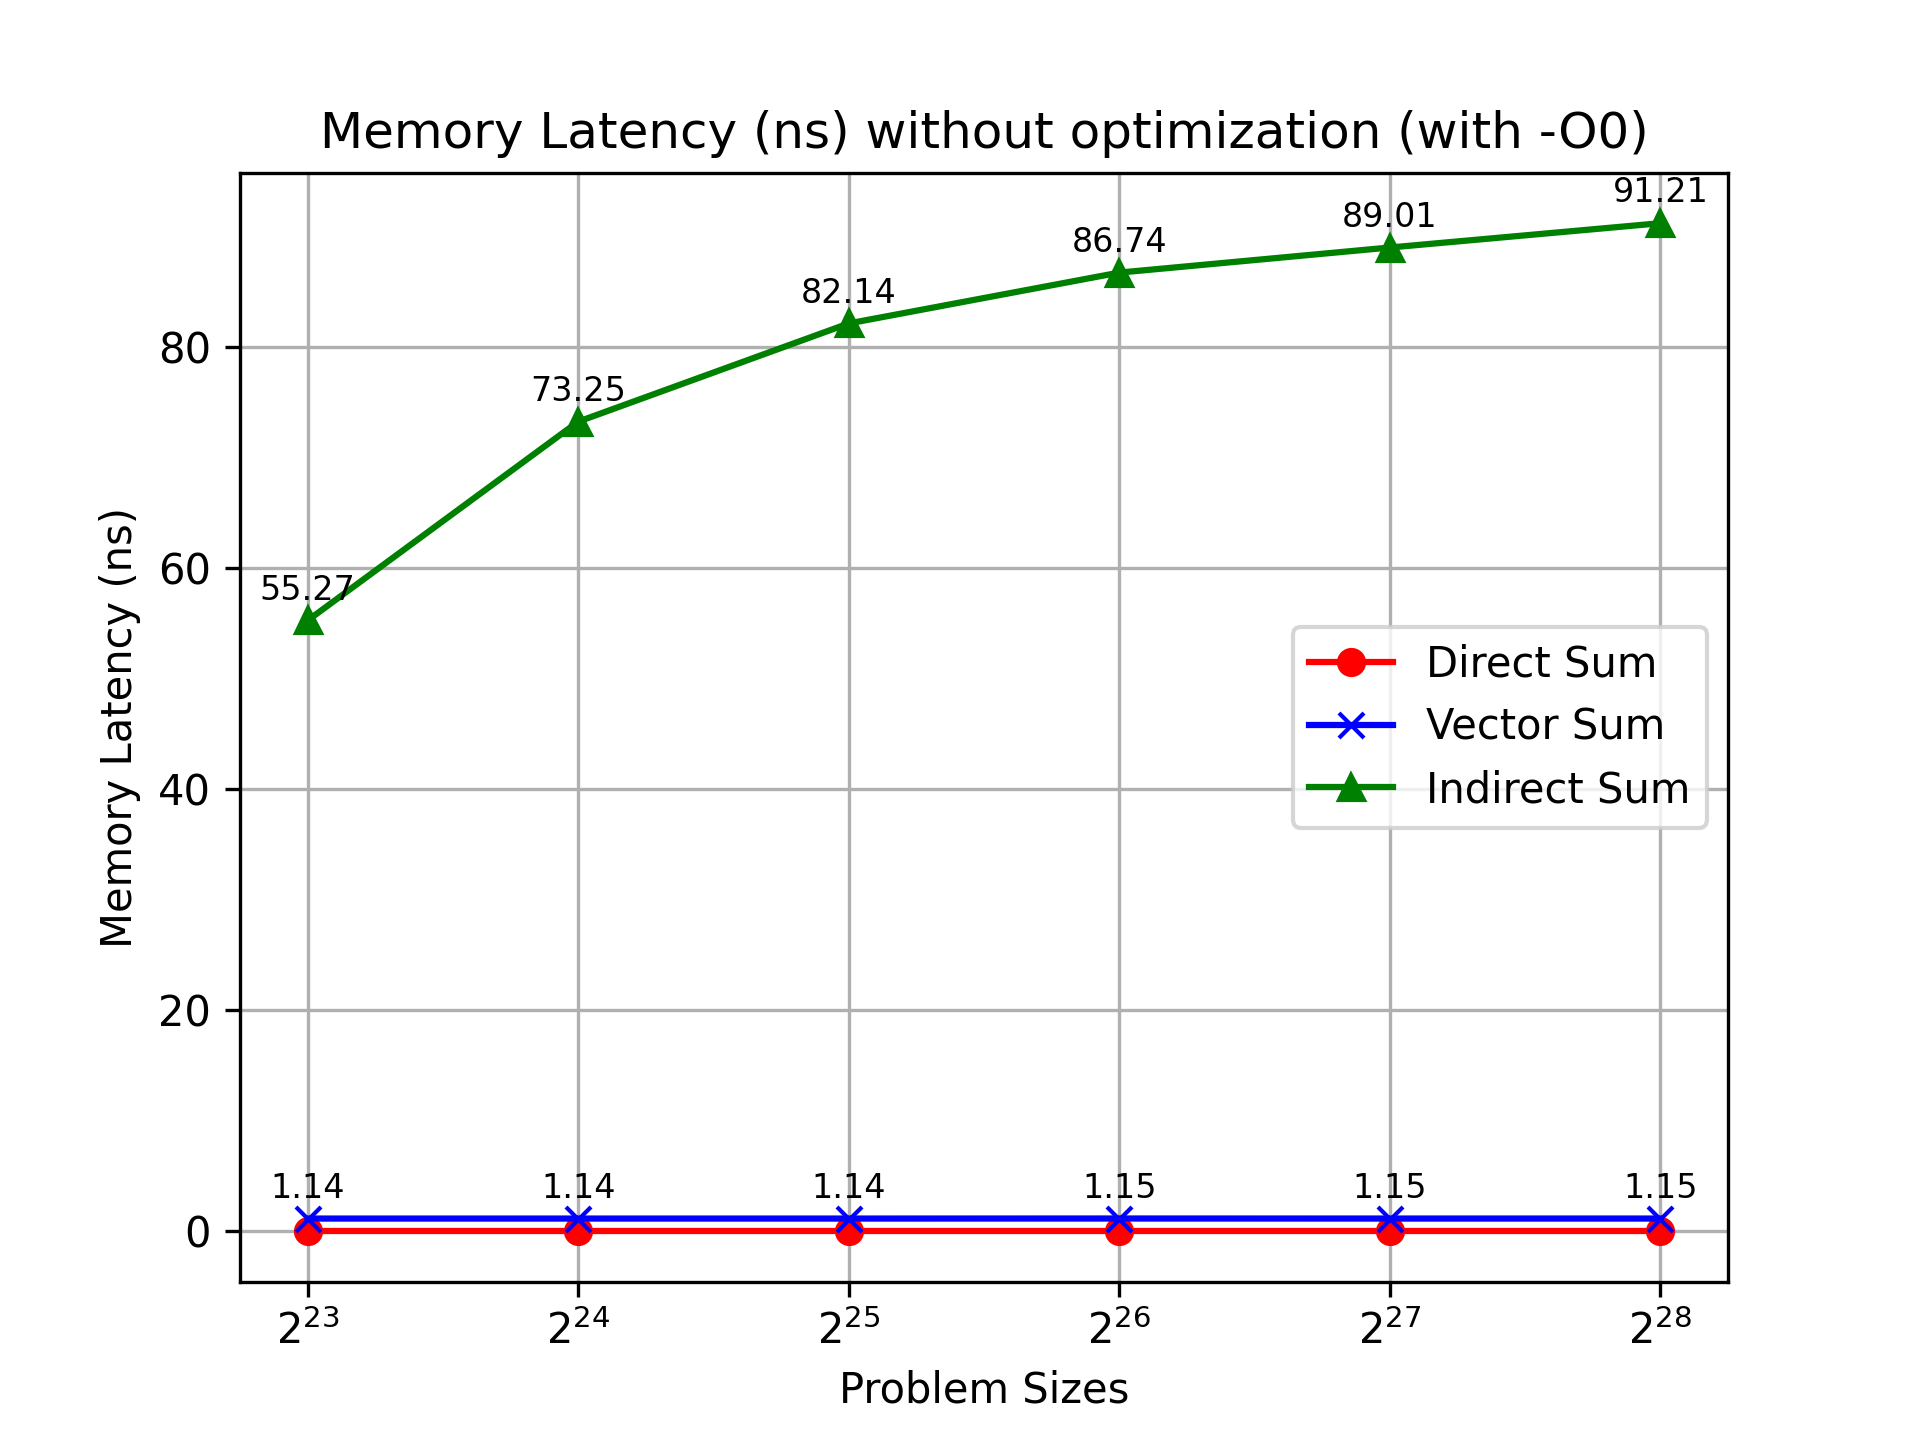
\includegraphics[width=0.45\textwidth]{Latency_O0.png}
    \caption{Estimated Memory Latency without optimization (\textit{-O0}).}
    \label{fig:Latency_O0}
\end{figure}

\begin{figure}[htbp]
    \centering
    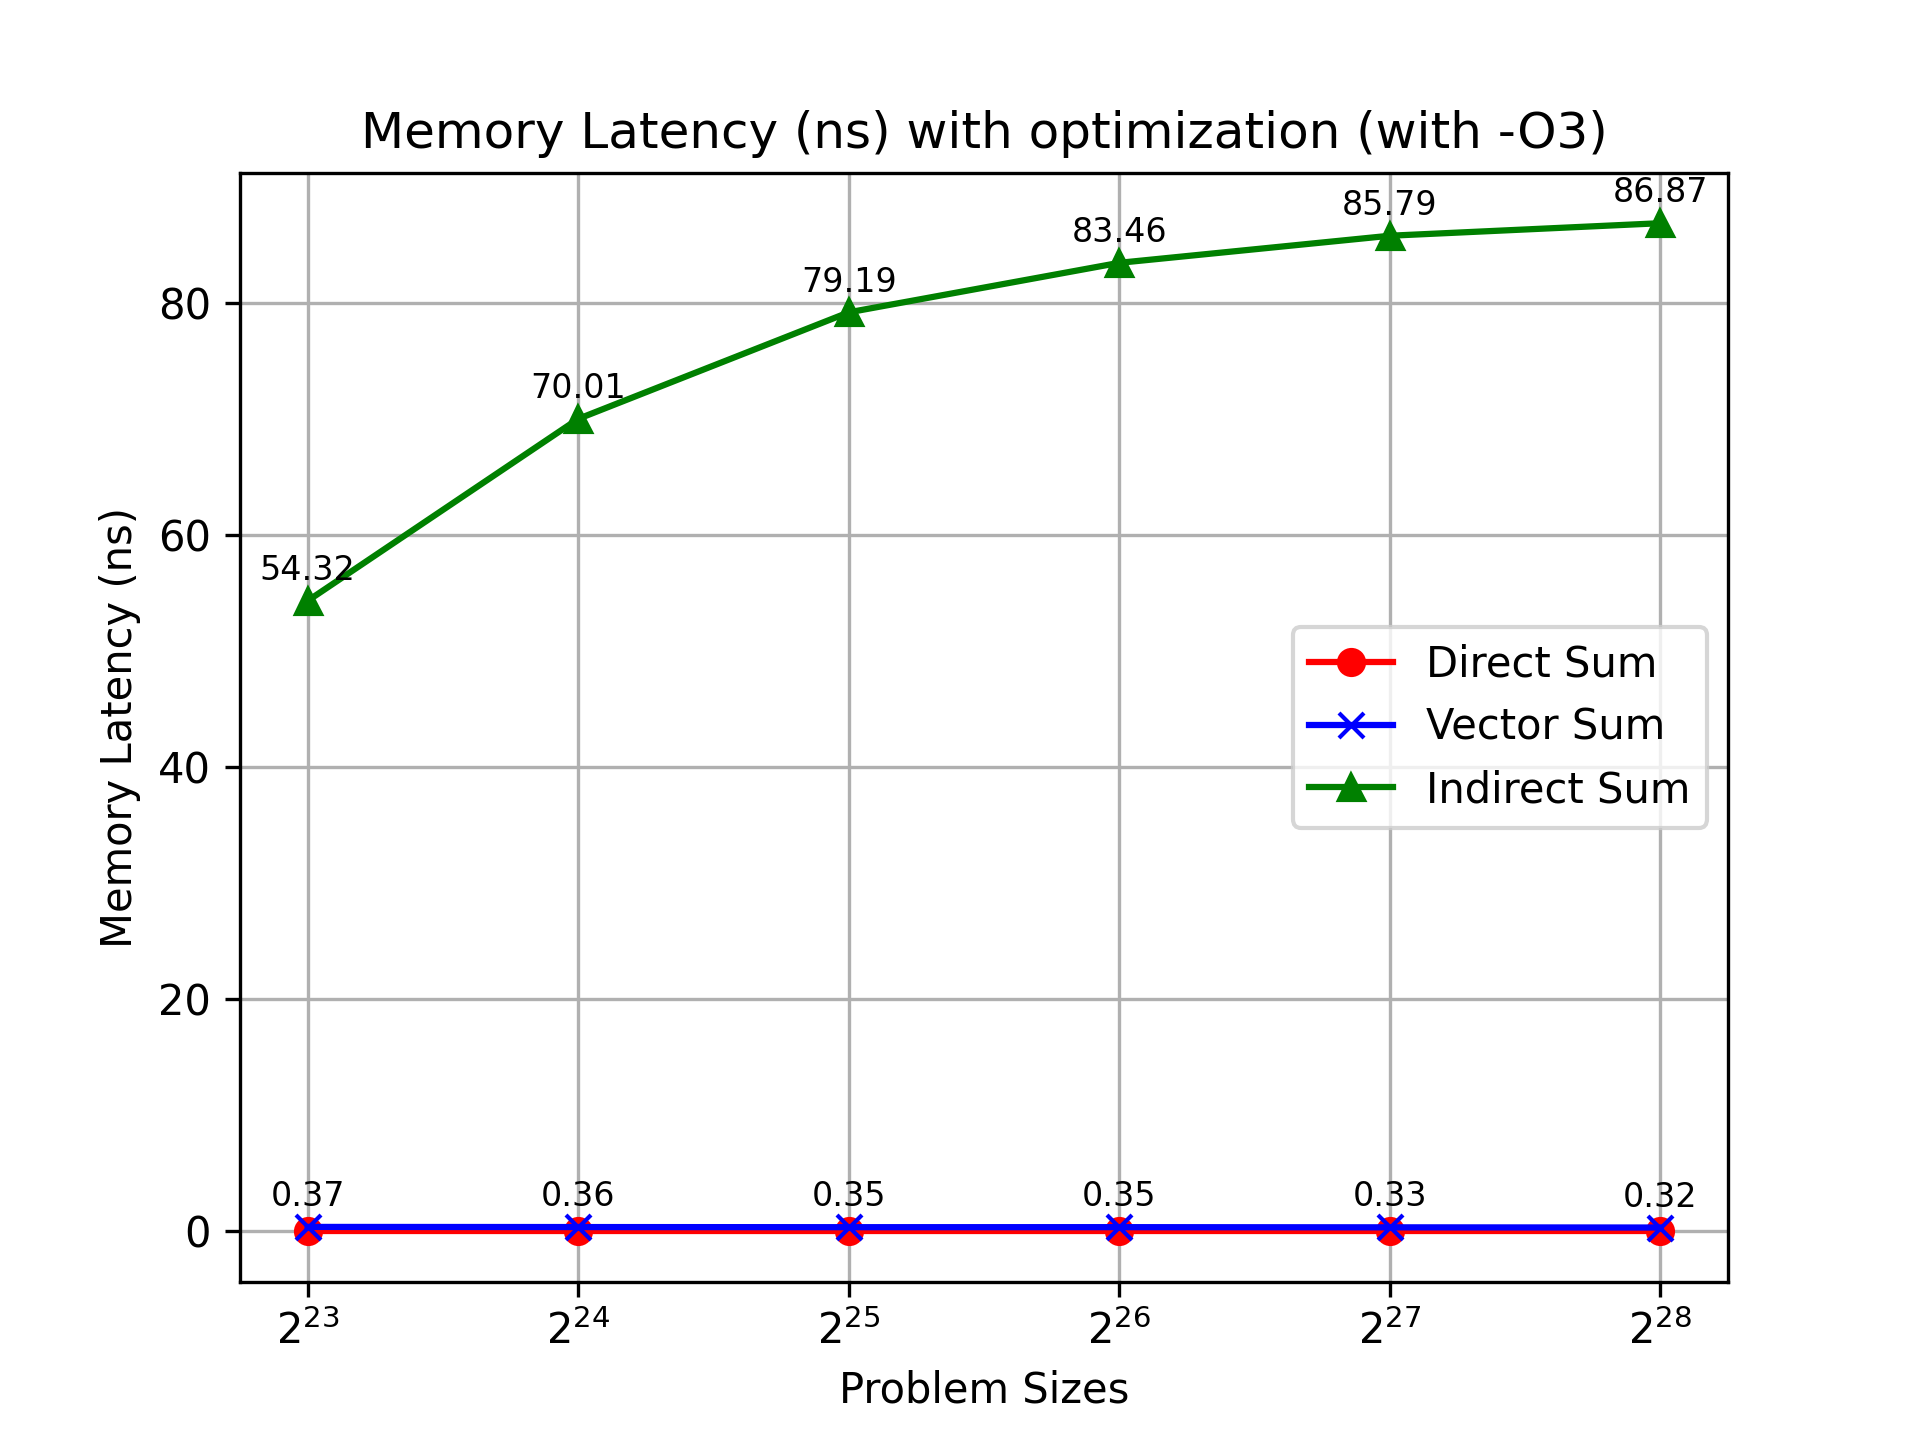
\includegraphics[width=0.45\textwidth]{Latency_O3.png}
    \caption{Estimated Memory Latency with optimization (\textit{-O3}).}
    \label{fig:Latency_O3}
\end{figure}

\begin{table}[htbp]
    \centering\small
    \begin{tabular}{c|cll}
 Problem Size (N) & Direct Sum (ns)& Vector Sum (ns)& Indirect Sum (ns)\\ \hline
 $2^{23}$ & 0.00& 1.14&55.27\\
 $2^{24}$ & 0.00& 1.14&73.25\\
 $2^{25}$ & 0.00& 1.14&82.14\\
 $2^{26}$ & 0.00& 1.15&86.74\\
 $2^{27}$ & 0.00& 1.15&89.01\\
 $2^{28}$ & 0.00& 1.15&91.21\\ 
    \end{tabular}
    \caption{Memory Latency without optimization (with \textit{-O0})}
    \label{tab:memory-latency-o0}
    \begin{tabular}{c|cll}
 Problem Size (N) & Direct Sum (ns)& Vector Sum (ns)& Indirect Sum (ns)\\ \hline
 $2^{23}$ & 0.00& 0.37&27.16\\
 $2^{24}$ & 0.00& 0.36&35.00\\
 $2^{25}$ & 0.00& 0.35&39.59\\
 $2^{26}$ & 0.00& 0.35&41.73\\
 $2^{27}$ & 0.00& 0.33&42.89\\
 $2^{28}$ & 0.00& 0.32&43.43\\ 
    \end{tabular}
    \caption{Memory Latency with optimization (with \textit{-O3})}
    \label{tab:memory-latency-o3}
\end{table}

\subsection{Findings and Discussion}

% In this section, please answer the questions posed in the homework assignment writeup on iLearn.

% Also, optionally include any additional insights you gained while doing these performance experiments.

% If this were an actual tech paper, here is where you would summarize the main findings and observations from the experiments: do the experiment results support your hypothesis? Sometimes the answer is a clear Y. Sometimes, the answer is Y for some circumstances, but not all, and it is important to spell this out.

% Sometimes, the experiments turn up unexpected negative results, and it is also important to point out those, as well. Science happens due to both successes and failures, and it is important to document failed experiments so that we can all learn from them.
\subsubsection{MFLOP/s}
% What is the number of FLOPs/second you are able to realize in this assignment? Which of the 3 programs are you using to derive this figure, and why? Suggest you create a table showing FLOPs/second for each of the 3 applications at each of the compiler optimization levels. How does your FLOPs/second rate compare to the theoretical peak for the AMD EPYC 7763 processors on Perlmutter  (Look here for more info)

The highest throughput achieved was 7,027.1 MFLOP/s with the direct sum method, which avoids memory access and thus is suitable for measuring pure computational throughput (see Table~\ref{tab:mflops-o3}). However, this is lower than the theoretical peak of 39.2 GFLOPS per core for the AMD EPYC 7763 processor (see Table~\ref{tab:machine_detail}).

This gap is due to several factors: the theoretical peak assumes full utilization of both threads per core and the AVX2 instruction set, which can perform eight single-precision operations per thread. The peak is calculated as \(2.45 \, \text{GHz} \times 2 \, \text{threads} \times 8 = 39.2 \, \text{GFLOPS}\). In contrast, our program uses only one thread, and the `vpaddq` SIMD instruction in the compiled code, which we observed in the disassembled program, allows only two computations per cycle, limiting performance.

\subsubsection{Memory Bandwidth}
% What is the min/max/average memory bandwidth you are able to realize in this assignment? And in which of the 3 programs does this happen, and why? Consider using a table to present min/max/avg memory bandwidth used across the different applications and different optimization levels. How do your memory bandwidth utilization numbers compare to the maximum theoretical peak on Perlmutter CPU nodes? (See link in previous bullet for reference information)
The minimum, maximum, and average memory bandwidth for each summation method are shown in Table~\ref{tab:min-max-avg-memory-bandwidth-o0} and Table~\ref{tab:min-max-avg-memory-bandwidth-o3}. The direct sum method consistently shows the minimum bandwidth as it does not access memory. In contrast, the vector sum method achieves the highest utilization due to its efficient use of sequential memory access, which enhances spatial locality. However, even the maximum observed bandwidth of 25.29 GB/s falls short of the system's theoretical peak of 204.8 GB/s (see Table~\ref{tab:machine_detail}). The program might not fully utilize the multiple memory channels available on the system because it runs on a single thread, which potentially underutilizes the 8 memory channels available per socket (see Table~\ref{tab:machine_detail}).

\begin{table}[htbp]
    \centering
    \begin{tabular}{c|cll}
 & Direct Sum & Vector Sum & Indirect Sum \\ \hline
 Min& 0.00& 6.96&0.09\\
 Max& 0.00& 6.99&0.14\\
 Avg& 0.00& 6.98&0.10\\ 
    \end{tabular}
    \caption{Min/Max/Average Memory Bandwidth Utilization (GB/s) without optimization (with \textit{-O0})}
    \label{tab:min-max-avg-memory-bandwidth-o0}
    \begin{tabular}{c|cll}
 & Direct Sum & Vector Sum & Indirect Sum \\ \hline
 Min& 0.00& 21.65&0.09\\
 Max& 0.00& 25.29&0.15\\
 Avg& 0.00& 23.23&0.11\\ 
    \end{tabular}
    \caption{Min/Max/Average  Memory Bandwidth Utilization (GB/s) with optimization (with \textit{-O3})}
    \label{tab:min-max-avg-memory-bandwidth-o3}
\end{table}


\subsubsection{Memory Latency}
% Which code configuration/problem size combination results in the lowest measured memory latency, and why? Which results in the highest measured memory latency, and why?

The estimated memory latency for each summation method is presented in Table~\ref{tab:memory-latency-o0} and Table~\ref{tab:memory-latency-o3}. The direct sum method has the lowest latency as it does not involve memory access. In contrast, the indirect sum with the largest problem size (\(2^{28}\)) compiled with the no-optimization flag (\textit{-O0}) shows the highest latency due to poor spatial locality from random memory accesses. As the problem size increases, cache hit rates decrease because cache lines are more likely to be evicted before being reused.

\subsubsection{Compiler Optimization}
The effects of compiler optimization (\textit{-O3}) are significant when there is no memory access (direct sum) or when memory access is efficient (vector sum). In these cases, the compiler can effectively optimize computational instructions, leading to noticeable performance improvements. However, for the indirect sum method, the impact of compiler optimization is minimal. This is because the performance gains from compiler optimizations are only a few nanoseconds per loop, whereas the cache miss penalty, caused by the lack of spatial locality, is approximately 100 nanoseconds per loop. As a result, the benefits of optimization are overshadowed by the higher cost of cache misses in the indirect sum method.